\documentclass[10pt,twocolumn]{article}

\usepackage[a4paper,margin=18mm,columnsep=7mm]{geometry}
\usepackage[T1]{fontenc}
\usepackage{newtxtext,newtxmath}
\usepackage{amsmath}
\usepackage{graphicx}
\usepackage{booktabs}
\usepackage{multirow}
\usepackage{xcolor}
\usepackage[font=small,labelfont=bf,skip=4pt]{caption}
\usepackage{subcaption}
\usepackage{algorithm}
\usepackage{algpseudocode}
\usepackage{tikz}
\usetikzlibrary{arrows.meta,positioning,fit,backgrounds}
\usepackage{enumitem}
\usepackage[numbers,sort&compress]{natbib}
\usepackage{titlesec}
\usepackage[colorlinks=true,linkcolor=blue!50!black,citecolor=blue!50!black,urlcolor=blue!50!black]{hyperref}

\graphicspath{{figures/}{../docs/figures/}}
\setlist{itemsep=1pt,topsep=3pt,leftmargin=*}
\titleformat{\section}{\normalfont\large\bfseries}{\thesection}{0.6em}{}
\titleformat{\subsection}{\normalfont\normalsize\bfseries}{\thesubsection}{0.6em}{}
\titlespacing*{\section}{0pt}{9pt}{4pt}
\titlespacing*{\subsection}{0pt}{7pt}{3pt}
\newcommand{\IG}{\mathrm{IG}}
\newcommand{\E}{\mathbb{E}}
\definecolor{accent}{HTML}{2B5797}
\definecolor{warn}{HTML}{B36B00}

\title{\Large\bfseries Attribution-Based Explanations of Neural Summary Networks\\[2pt]
in Amortized Simulation-Based Inference}
\author{Feriha Bircan\\[2pt]
\small Research internship project\\
\small\url{https://github.com/ferihabircan/bayesflow-xai}}
\date{October 2026}

\begin{document}

\twocolumn[
\begin{@twocolumnfalse}
\maketitle
\vspace{-4mm}
\begin{abstract}
\noindent
Amortized Bayesian inference with BayesFlow compresses raw simulator output into a learned summary vector
before a conditional normalizing flow maps it to a posterior distribution. Whether this summary is built from
the physically meaningful part of the data is usually assessed only indirectly, through parameter recovery and
simulation-based calibration. We study four post-hoc attribution methods (Integrated Gradients, Saliency
Maps, Attention Rollout and Masking/Occlusion) applied to summary-network architectures trained on four
simulators of increasing complexity: a stationary SIR epidemic model, a sinusoidal toy signal with known
ground truth, a Gaussian random field, and a gravitational-wave benchmark. Gradient-based attribution is made
possible by surrogate regressors that share the summary network's architecture, and all combinations are run
through a single configuration-driven plugin registry. On the toy signal, Integrated Gradients recovers the
known ground truth in 188 of 200 samples. On the gravitational-wave benchmark it reveals that a network
trained on min-max-normalized strain ignores the merger and relies on a non-physical ${\sim}20$\,Hz artefact
introduced by the simulator's whitening step; switching to z-score normalization moves the attribution onto
the merger and reduces validation error from 9.27 to 1.41. On one trained model, Integrated Gradients and
Masking agree closely (rank correlation 0.99), whereas Saliency places 58\% of its mass in signal-free regions.
The SIR experiments delimit the approach: methods disagree on the relevant input channel, and the recurrent
read-out and the attribution baseline leave identifiable fingerprints on the maps.
\end{abstract}
\vspace{5mm}
\end{@twocolumnfalse}
]

%======================================================================
\section{Introduction}
%======================================================================

Many scientific models are available only as stochastic simulators: given parameters $\theta$ one can sample
data $x\sim p(x\mid\theta)$, but the likelihood cannot be evaluated. Simulation-based inference
(SBI)~\cite{cranmer2020frontier} replaces likelihood evaluations by learning from simulated pairs
$(\theta,x)$. Neural posterior estimation~\cite{papamakarios2016fast,greenberg2019automatic}, as implemented in
BayesFlow~\cite{radev2020bayesflow,radev2023bayesflow}, trains a \emph{summary network} that compresses a data set
into a fixed-size vector jointly with a conditional normalizing flow that represents the posterior. Once
trained, inference on a new data set requires a single forward pass; the training cost is \emph{amortized}
over all future data sets.

The reliability of such estimators is normally established with loss curves, parameter recovery and
simulation-based calibration (SBC)~\cite{talts2018sbc}. These diagnostics show whether the posterior is
accurate \emph{on simulated data}; they do not show \emph{which features} of the data the network relies on. A
network can reach a low loss by exploiting a property of the simulator that real observations will not have,
and posterior approximations can be unfaithful in ways that standard training metrics do not expose~\cite{hermans2022trust}.

Feature-attribution methods from explainable AI (XAI) assign an importance score to every input element for a
given network output~\cite{simonyan2014deep,sundararajan2017axiomatic,zeiler2014visualizing,abnar2020quantifying}.
They are widely used for image classifiers but rarely for the summary networks of amortized SBI. We ask:

\begin{enumerate}[label=\textbf{Q\arabic*}]
  \item Do attributions recover what is known to be informative when the ground truth is known?
  \item Do different attribution methods agree on the same trained model?
  \item Can attributions reveal problems that standard SBI diagnostics miss?
\end{enumerate}

\paragraph{Contributions.}
(i)~An open-source plugin registry in which simulators, summary networks, inference networks and attribution
methods are registered by name and combined from a configuration file.
(ii)~A study of four attribution methods on four simulators, including a gravitational-wave benchmark from the
SBI literature~\cite{deistler2025practical}.
(iii)~Evidence that attribution exposes a simulator artefact on that benchmark, which the network trained with
the original normalization relies on, together with a quantitative comparison of three methods on one model.

%======================================================================
\section{Related Work}
%======================================================================

\paragraph{Amortized and neural SBI.}
Neural posterior estimation learns $q(\theta\mid x)$ directly from simulations~\cite{papamakarios2016fast,greenberg2019automatic};
BayesFlow~\cite{radev2020bayesflow,radev2023bayesflow} couples learned summary statistics with invertible
networks~\cite{dinh2017realnvp,durkan2019neural}, and has been applied, among others, to epidemiological
models~\cite{radev2021outbreakflow}. In gravitational-wave astronomy, neural posterior estimation enables
real-time parameter inference~\cite{dax2021realtime}. Validation relies on calibration checks such as
SBC~\cite{talts2018sbc}, and Hermans et al.~\cite{hermans2022trust} showed that SBI posteriors can be
overconfident, motivating additional diagnostics.

\paragraph{Feature attribution.}
Gradient-based methods range from raw input gradients~\cite{simonyan2014deep} to path-integrated
gradients~\cite{sundararajan2017axiomatic}; perturbation-based methods occlude input regions~\cite{zeiler2014visualizing};
model-agnostic surrogates include LIME~\cite{ribeiro2016lime} and SHAP~\cite{lundberg2017shap}. For
Transformers, attention rollout propagates attention through layers~\cite{abnar2020quantifying}. Several
studies show that attributions can be unreliable: saliency maps may be insensitive to the model
parameters~\cite{adebayo2018sanity}, depend on input shifts~\cite{kindermans2019unreliability}, and, for
path methods, strongly on the choice of baseline~\cite{sturmfels2020baselines}. Ancona et al.~\cite{ancona2018towards}
relate gradient-based methods formally. Our study takes these caveats into the SBI setting and uses agreement
between methods and known ground truth as sanity checks.

%======================================================================
\section{Background}
%======================================================================

\subsection{Amortized posterior estimation}

Let $s_\psi$ denote the summary network and $q_\phi(\theta\mid s)$ a conditional normalizing flow. BayesFlow
minimizes the expected negative log posterior density over the joint distribution of parameters and data,
\begin{equation}
  \min_{\psi,\phi}\;\E_{p(\theta)\,p(x\mid\theta)}\!\left[-\log q_\phi\big(\theta \,\big|\, s_\psi(x)\big)\right].
  \label{eq:npe}
\end{equation}
At the optimum, $q_\phi(\theta\mid s_\psi(x))$ equals the true posterior provided that $s_\psi(x)$ is a
sufficient summary. \emph{Parameter recovery} compares posterior point estimates with the ground truth on
held-out simulations; \emph{SBC} checks that the rank of the true parameter among posterior draws is uniform,
as it must be for a calibrated posterior~\cite{talts2018sbc}.

\subsection{Attribution methods}

Let $f:\mathbb{R}^d\to\mathbb{R}$ be a scalar model output and $x'$ a baseline input.

\emph{Saliency}~\cite{simonyan2014deep} is the absolute input gradient,
\begin{equation}
  S_i(x) = \left|\partial f(x) / \partial x_i\right|,
\end{equation}
a measure of local \emph{sensitivity}.

\emph{Integrated Gradients} (IG)~\cite{sundararajan2017axiomatic} integrates the gradient along the straight
path from $x'$ to $x$:
\begin{equation}
  \IG_i(x) = (x_i - x'_i)\int_0^1 \frac{\partial f\big(x' + \alpha(x-x')\big)}{\partial x_i}\,d\alpha .
  \label{eq:ig}
\end{equation}
IG satisfies \emph{completeness}, $\sum_i \IG_i(x) = f(x) - f(x')$. The integral is approximated by a Riemann
sum with $n$ steps, and the \emph{convergence delta} $\delta = |\sum_i \IG_i - (f(x)-f(x'))|$ quantifies the
approximation error. Because of the factor $(x_i-x'_i)$, IG measures \emph{contribution relative to the
baseline}.

\emph{Attention Rollout}~\cite{abnar2020quantifying} combines head-averaged attention matrices $A^{(l)}$ of
$L$ layers with the identity, which accounts for residual connections:
\begin{equation}
  \tilde A = \prod_{l=1}^{L} \operatorname{norm}\!\Big(\tfrac12 A^{(l)} + \tfrac12 I\Big),
\end{equation}
where $\operatorname{norm}$ renormalizes rows to sum to one.

\emph{Masking (occlusion)}~\cite{zeiler2014visualizing} replaces a region $R$ by the baseline and records
\begin{equation}
  M_R(x) = \big|f(x) - f(x_{R\leftarrow x'})\big| ,
\end{equation}
which needs one forward pass per region and no gradients.

%======================================================================
\section{Method}
%======================================================================

\begin{figure}[t]
\centering
\resizebox{\columnwidth}{!}{%
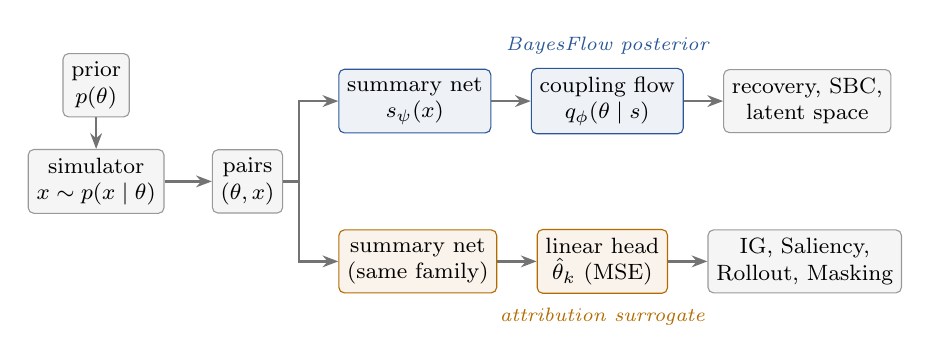
\begin{tikzpicture}[
  node distance=4mm and 5mm,
  box/.style={draw=black!40, rounded corners=2pt, fill=black!4, align=center, font=\footnotesize, minimum height=8mm, inner sep=3pt},
  bf/.style={box, draw=accent, fill=accent!8},
  xai/.style={box, draw=warn, fill=warn!8},
  arr/.style={-{Stealth[length=2mm]}, black!55, thick}]
  \node[box] (prior) {prior\\$p(\theta)$};
  \node[box, below=of prior] (sim) {simulator\\$x\sim p(x\mid\theta)$};
  \node[box, right=6mm of sim] (pairs) {pairs\\$(\theta,x)$};
  \node[bf, above right=2mm and 7mm of pairs] (sbf) {summary net\\$s_\psi(x)$};
  \node[bf, right=of sbf] (flow) {coupling flow\\$q_\phi(\theta\mid s)$};
  \node[box, right=of flow] (diag) {recovery, SBC,\\latent space};
  \node[xai, below right=2mm and 7mm of pairs] (sxai) {summary net\\(same family)};
  \node[xai, right=of sxai] (head) {linear head\\$\hat\theta_k$ (MSE)};
  \node[box, right=of head] (attr) {IG, Saliency,\\Rollout, Masking};
  \draw[arr] (prior) -- (sim);
  \draw[arr] (sim) -- (pairs);
  \draw[arr] (pairs.east) -- ++(2mm,0) |- (sbf.west);
  \draw[arr] (pairs.east) -- ++(2mm,0) |- (sxai.west);
  \draw[arr] (sbf) -- (flow); \draw[arr] (flow) -- (diag);
  \draw[arr] (sxai) -- (head); \draw[arr] (head) -- (attr);
  \node[font=\scriptsize\itshape, text=accent, above=0.5mm of flow] {BayesFlow posterior};
  \node[font=\scriptsize\itshape, text=warn, below=0.5mm of head] {attribution surrogate};
\end{tikzpicture}}
\caption{Pipeline. Each simulator trains a BayesFlow posterior, evaluated with the standard diagnostics, and a
surrogate regressor of the same summary-network family, on which attribution methods are computed.}
\label{fig:pipeline}
\end{figure}

\subsection{Posterior estimators and attribution surrogates}

For every simulator we train two models (Fig.~\ref{fig:pipeline}). The \emph{BayesFlow posterior} optimizes
Eq.~\eqref{eq:npe} and is evaluated with recovery and SBC; the latent-space projection (UMAP and t-SNE of
summary vectors) is computed on its summary network. The \emph{attribution surrogate} is a plain PyTorch summary
network of the same family followed by a linear head, trained with mean-squared error to predict all
parameters. A wrapper exposes a single output $f(x)=\hat\theta_k(x)$ for the target parameter $k$, as required
by Captum~\cite{kokhlikyan2020captum}. The surrogate is needed because the flow's output is a distribution, not a
differentiable scalar. \textbf{All attribution maps therefore describe what a network of the given architecture
learns to extract from the data, not the normalizing-flow posterior itself.} Algorithm~\ref{alg:xai} summarizes
the procedure.

\begin{algorithm}[t]
\caption{Attribution analysis for a registered simulator}
\label{alg:xai}
\small
\begin{algorithmic}[1]
\Require simulator $\mathcal{S}$, summary-net builder $\mathcal{B}$, method $\mathcal{M}$, target index $k$
\State Simulate $\{(\theta^{(j)},x^{(j)})\}_{j=1}^{n}$ with $\mathcal{S}$; hold out 10\%
\State $g \gets \mathcal{B}(\mathcal{S})$; \; $h \gets$ linear layer
\State Train $(g,h)$ by Adam on $\sum_j\|h(g(x^{(j)}))-\theta^{(j)}\|^2$
\State $f(x) \gets [h(g(x))]_k$
\For{each validation input $x$}
  \State $a(x)\gets \mathcal{M}(f, x, x')$ \Comment{IG, Saliency, Rollout or Masking}
\EndFor
\State Aggregate $|a|$ over samples, channels or time; plot
\end{algorithmic}
\end{algorithm}

\subsection{Registry}

The package \texttt{bayesflow\_xai.registry} holds four dictionaries of simulators, summary networks, inference
networks and attribution methods, populated by decorators. A simulator is described by its parameter names,
input kind (time series or image), a dataset builder and shape information. A YAML file selects one entry from
each registry; \texttt{scripts/run\_workflow.py} trains the surrogate (Adam, learning rate $10^{-3}$) and runs the
selected method. Adding a simulator or method requires only a decorated function.

\subsection{Simulators}

\paragraph{SIR epidemic.} The stationary SIR model of the BayesFlow tutorial~\cite{radev2021outbreakflow}, in
discrete time with population $N=83\cdot10^6$:
\begin{equation}
\begin{aligned}
  C_t &= \lambda I_t S_t/N, & S_{t+1} &= S_t - C_t,\\
  I_{t+1} &= I_t + C_t - \mu I_t, & R_{t+1} &= R_t + \mu I_t .
\end{aligned}
\end{equation}
Reported cases over $T=60$ days start after a delay $D$ and follow a negative binomial with mean $C_t$ and
dispersion $\psi$. Priors: $\lambda\sim\mathrm{LogN}(\log 0.4,0.5)$, $\mu\sim\mathrm{LogN}(\log\tfrac18,0.2)$,
$D\sim\mathrm{LogN}(\log 8,0.2)$, $I_0\sim\Gamma(2,20)$, $\psi\sim\mathrm{Exp}$ with mean 5. The posterior sees
$\log(1+\text{cases})$; the surrogates see the noise-free fractions $(S,I,R)/N\in\mathbb{R}^{60\times3}$ and regress
$\log(1+\theta)$.

\paragraph{Toy signal (``Lotka--Volterra-style'').} Despite its name, not the predator--prey ODE: with
$\theta\sim\mathcal{U}(-1,1)^3$ and 20 time points $t\in[0,1]$,
\begin{equation}
  X_k(t)=\theta_{k-1}\sin\!\big(2\pi t(1+\theta_2)\big)+0.05\,\varepsilon,\quad k\in\{1,2\}.
\end{equation}
Thus $\theta_0$ affects only $X_1$: a ground truth for attribution.

\paragraph{Gaussian random field (GRF).} A $64\times64$ field with power spectrum $P(k)=k^{-\alpha}\sigma^2$,
$\log\sigma\sim\mathcal{N}(0,1)$, $\alpha\sim\mathcal{N}(4,0.5)$, from the BayesFlow spatial-data
example. The repository also reproduces the example's conditional diffusion model that generates fields.

\paragraph{Gravitational wave (GW).} The original benchmark simulator of the SBI practical
guide~\cite{deistler2025practical}, vendored unchanged: a binary black-hole merger (PyCBC, IMRPhenomPv2) with
$m_1\sim\mathcal{U}(40,80)$ and $q=m_2/m_1\sim\mathcal{U}(0.25,0.99)$, projected onto the LIGO H1 and L1
detectors, with simulated noise, whitened and high-passed at 20\,Hz; 4\,s at 2048\,Hz (8192 samples per
detector), aligned so that the H1 merger is at $t=0$. The target is $m_1$.

\subsection{Architectures and settings}

Table~\ref{tab:setup} lists the networks and training budgets. IG uses a zero baseline with $n=50$ steps for SIR,
the toy signal and the GRF, and the zero-strain level (the median input) with $n=200$ for GW. Masking occludes
single time steps (all channels) or $8\times8$ patches with zeros; for GW it occludes 32-sample (15.6\,ms)
windows of one detector at a time. For the SIR and toy-signal statistics the first and last time step are
excluded from importance rankings (Sec.~\ref{sec:fingerprints}).

\begin{table}[t]
\centering
\caption{Summary networks and training budgets of the attribution surrogates (and the BayesFlow posteriors).}
\label{tab:setup}
\footnotesize
\setlength{\tabcolsep}{3.5pt}
\begin{tabular}{@{}llll@{}}
\toprule
Simulator & Summary network & Sims & Epochs \\
\midrule
SIR & GRU (64 units, 8-dim) & 6000 & 60 \\
    & Transformer ($d{=}32$, 4 heads, 2 layers) & 4000 & 60 \\
    & \textit{BayesFlow: GRU + spline flow} & \textit{6000} & \textit{100} \\
Toy signal & GRU (64 units, 8-dim) & 6000 & 60 \\
GRF & CNN (widths 8--64, 6-dim) & 2000 & 30 \\
    & \textit{BayesFlow: CNN + coupling flow} & \textit{online} & \textit{20} \\
GW & dilated CNN, 13 layers~\cite{hermans2022trust} & 5000 & 40 \\
\bottomrule
\end{tabular}
\end{table}

%======================================================================
\section{Experiments and Results}
%======================================================================

All numbers below are taken from the figures, logs and summaries in the repository. Training times on one
NVIDIA RTX 2080 Ti were 8.9\,min (SIR posterior), 44\,min (GRF posterior) and 89\,min (GRF diffusion model).

\subsection{Posterior quality}

\begin{figure*}[t]
\centering
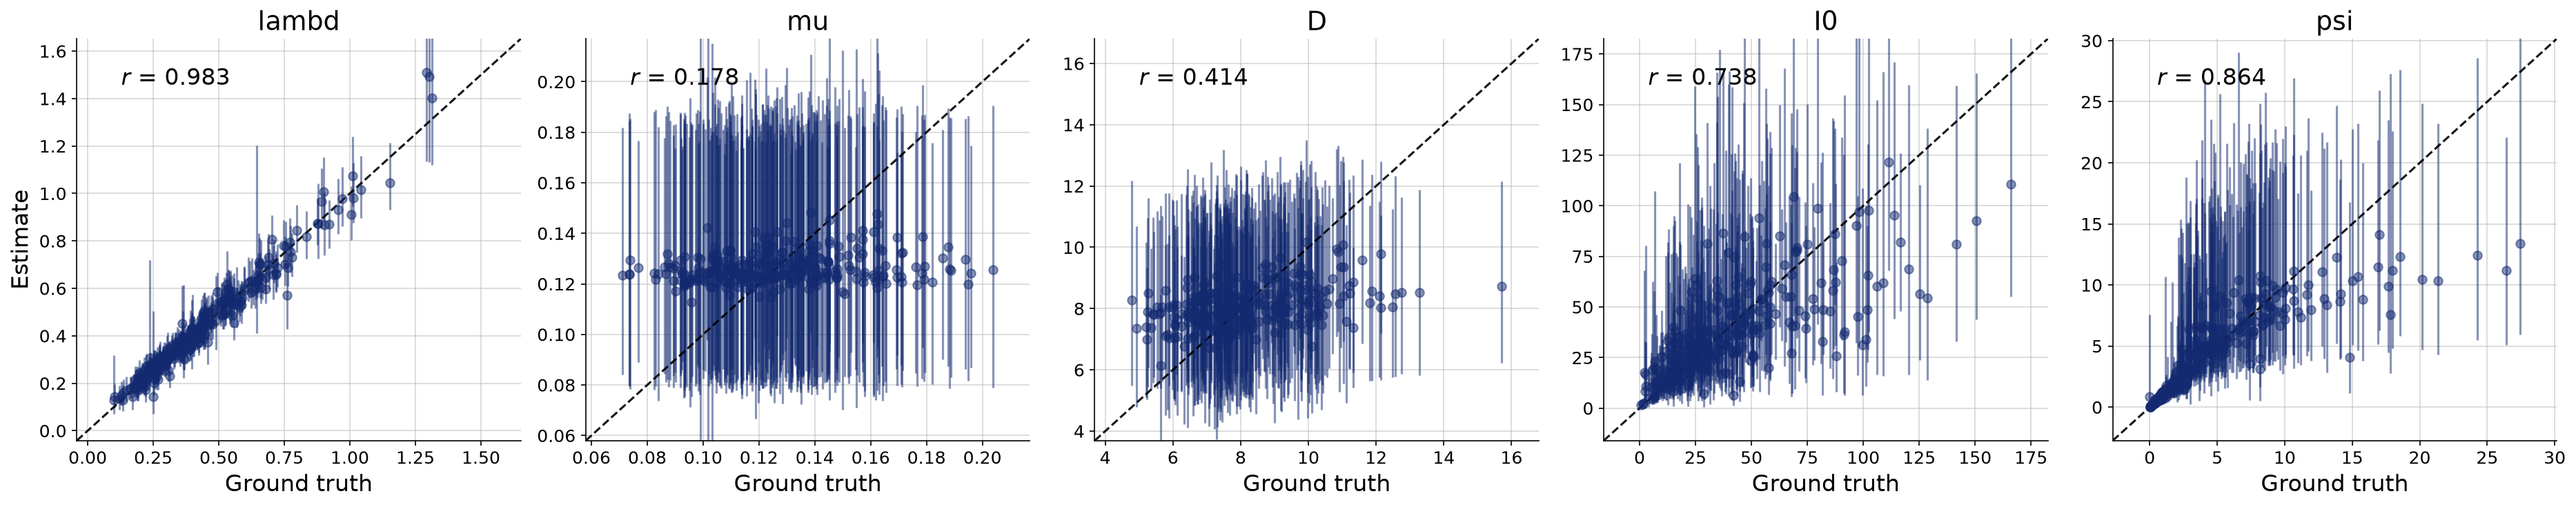
\includegraphics[width=0.8\textwidth]{sir/02_parameter_recovery.png}\\[0.5mm]
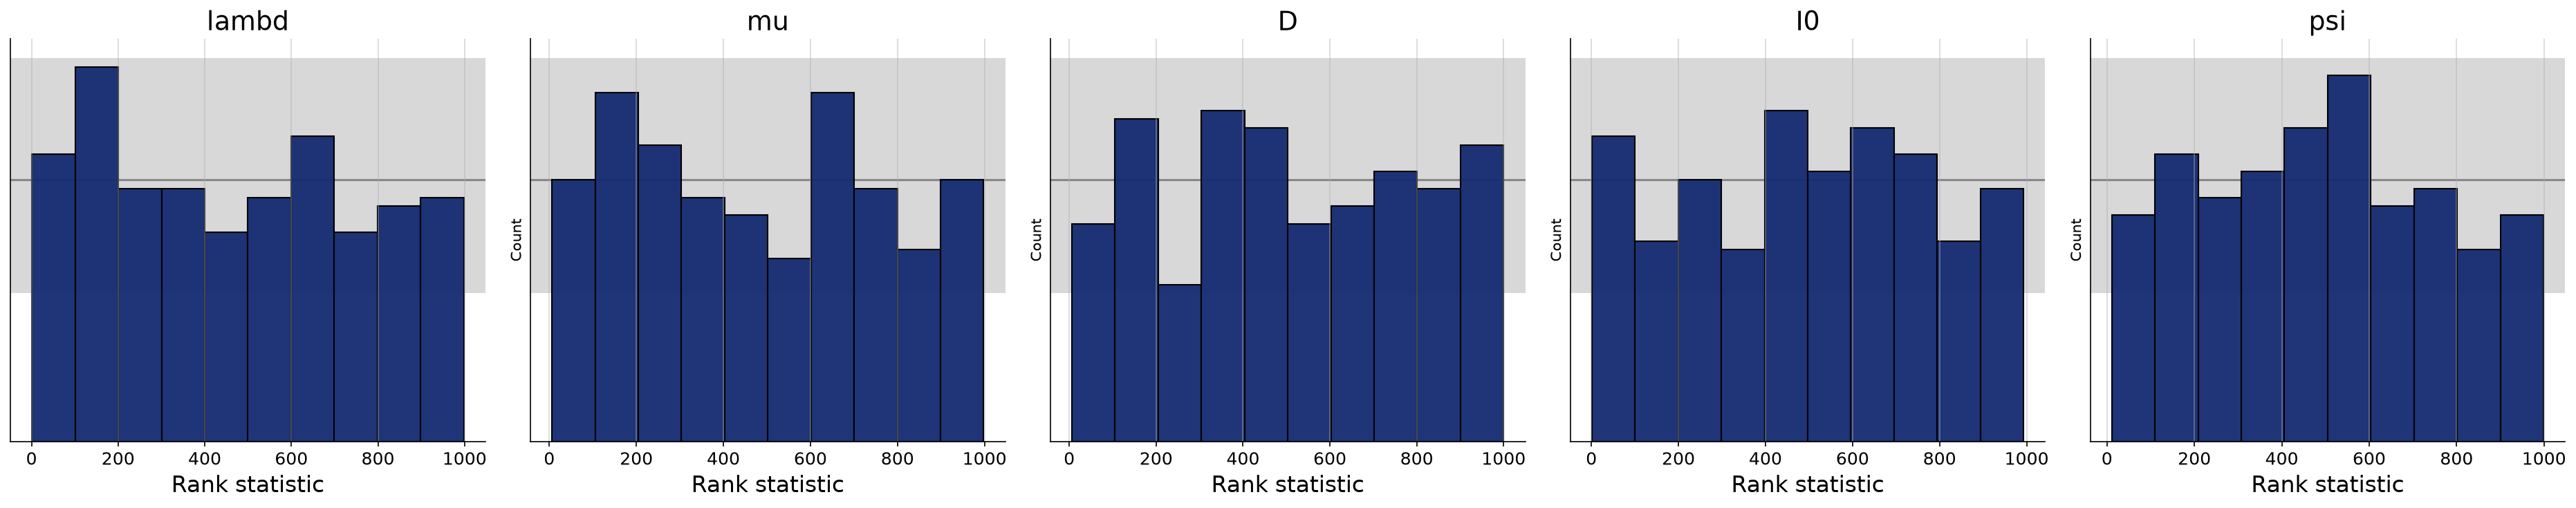
\includegraphics[width=0.8\textwidth]{sir/03_sbc_calibration.png}
\caption{BayesFlow posterior for SIR on 300 held-out data sets (1000 draws each). \textbf{Top:} posterior median
versus ground truth with posterior intervals. \textbf{Bottom:} SBC rank histograms; bars inside the grey band are
consistent with calibration.}
\label{fig:sir-diag}
\end{figure*}

For SIR (Fig.~\ref{fig:sir-diag}), recovery is near-perfect for the infection rate $\lambda$ ($r=0.98$), good for
$\psi$ ($0.86$) and $I_0$ ($0.74$), and weak for $\mu$ ($0.18$) and $D$ ($0.41$), whose posteriors remain wide, as
expected for weakly identified parameters. All SBC histograms lie inside the confidence band. The UMAP and t-SNE
embeddings of 2000 summary vectors form a one-dimensional curve ordered by $\lambda$. For the GRF, recovery is
near-perfect ($r=0.999$ for $\log\sigma$, $0.993$ for $\alpha$) and the ECDF calibration curves stay inside the
95\% band.

\subsection{Surrogate fit}

Attributions are only meaningful for parameters the surrogate predicts. Table~\ref{tab:r2} reports held-out
$R^2$, recomputed on CPU with the repository's code and seeds. The SIR surrogate learns only $\lambda$: its
targets are not standardized, so the loss is dominated by $I_0$ and $\psi$ (variance ${\approx}0.6$ each on the
$\log(1+\cdot)$ scale), and $\psi$ is not identifiable from noise-free trajectories at all. All SIR explanations
therefore target $\lambda$.

\begin{table}[t]
\centering
\caption{Held-out $R^2$ of the GRU surrogates.}
\label{tab:r2}
\footnotesize
\begin{tabular}{@{}lccccc@{}}
\toprule
SIR & $\lambda$ & $\mu$ & $D$ & $I_0$ & $\psi$ \\
 & \textbf{0.90} & $-1.16$ & 0.02 & 0.03 & $-0.01$ \\
\midrule
Toy signal & $\theta_0$ & $\theta_1$ & $\theta_2$ & & \\
 & \textbf{0.98} & \textbf{0.99} & \textbf{0.97} & & \\
\bottomrule
\end{tabular}
\end{table}

\subsection{Q1: Recovering a known ground truth}

\begin{figure}[t]
\centering
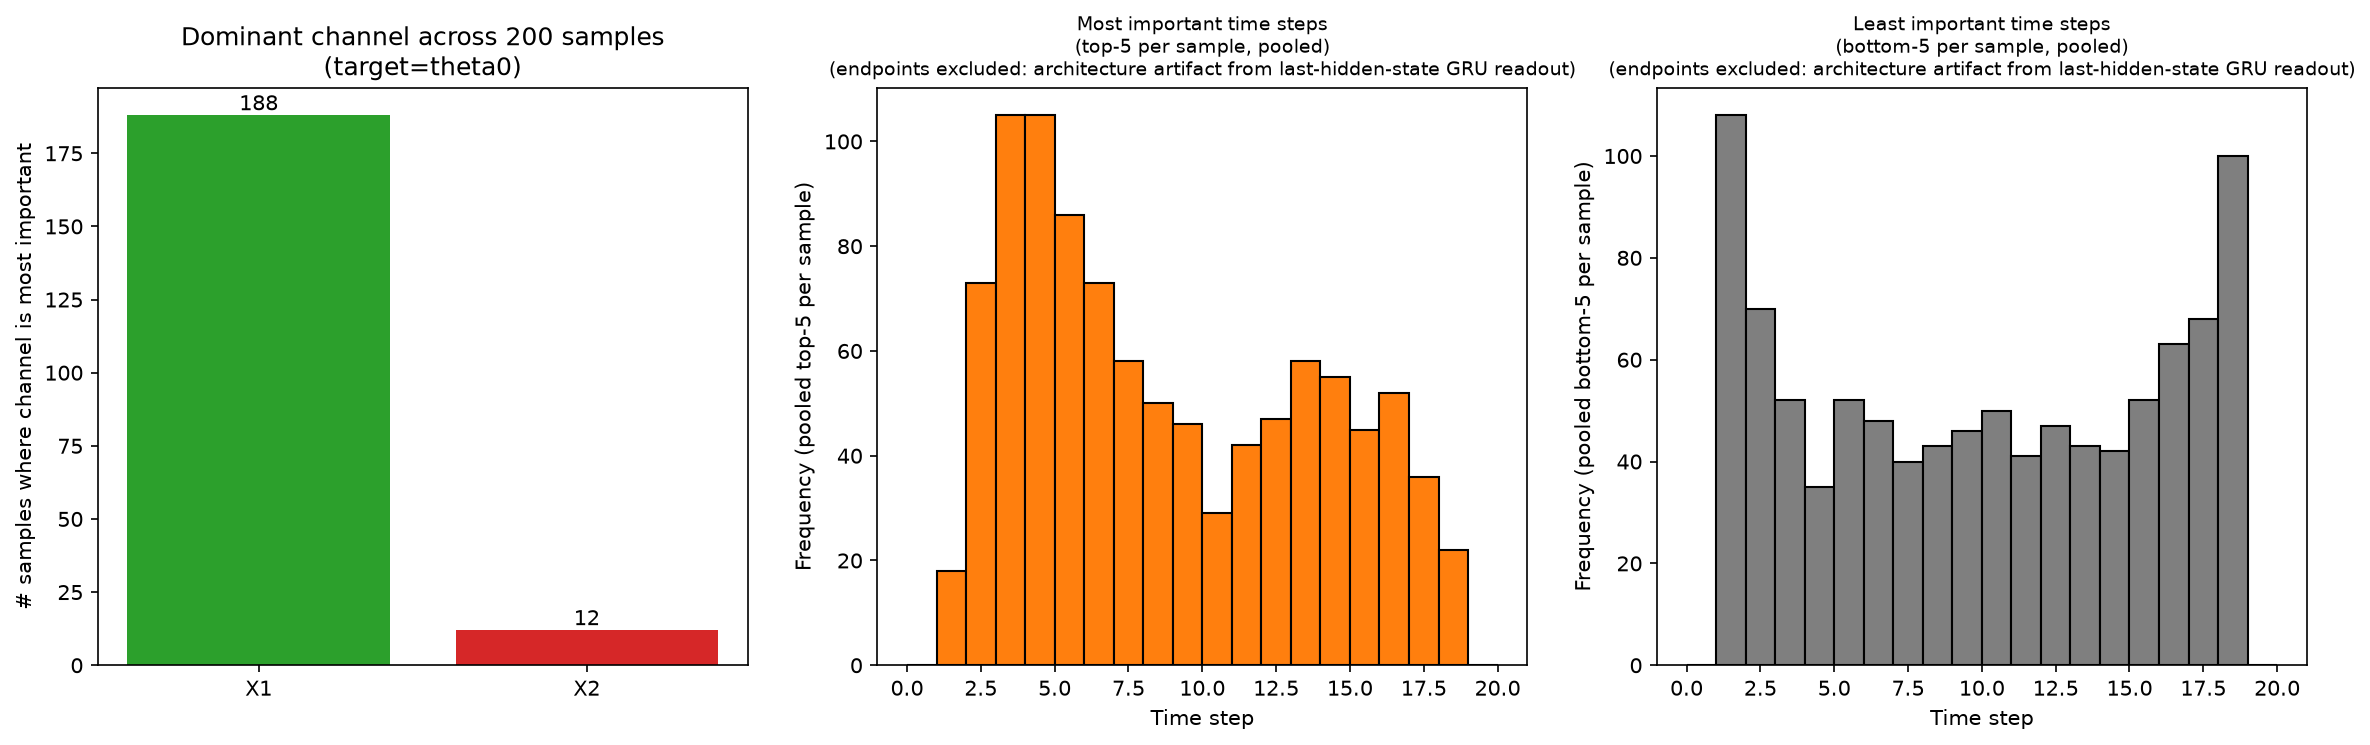
\includegraphics[width=\columnwidth]{lotka_volterra/xai_lv_04_channel_time_importance_stats.png}
\caption{Toy signal, IG for target $\theta_0$ over 200 validation samples. \textbf{Left:} dominant channel per
sample; $\theta_0$ scales only $X_1$ by construction. \textbf{Middle/right:} pooled top-5 and bottom-5 interior
time steps per sample.}
\label{fig:lv}
\end{figure}

For $\theta_0$, IG assigns the larger total attribution to $X_1$ in \textbf{188 of 200} samples
(Fig.~\ref{fig:lv}). The most important interior time steps cluster at steps 3--6 and 13--17, around the extrema
of the sine, where the amplitude is easiest to read.

\subsection{Q2: Agreement between methods on SIR}

\begin{figure}[t]
\centering
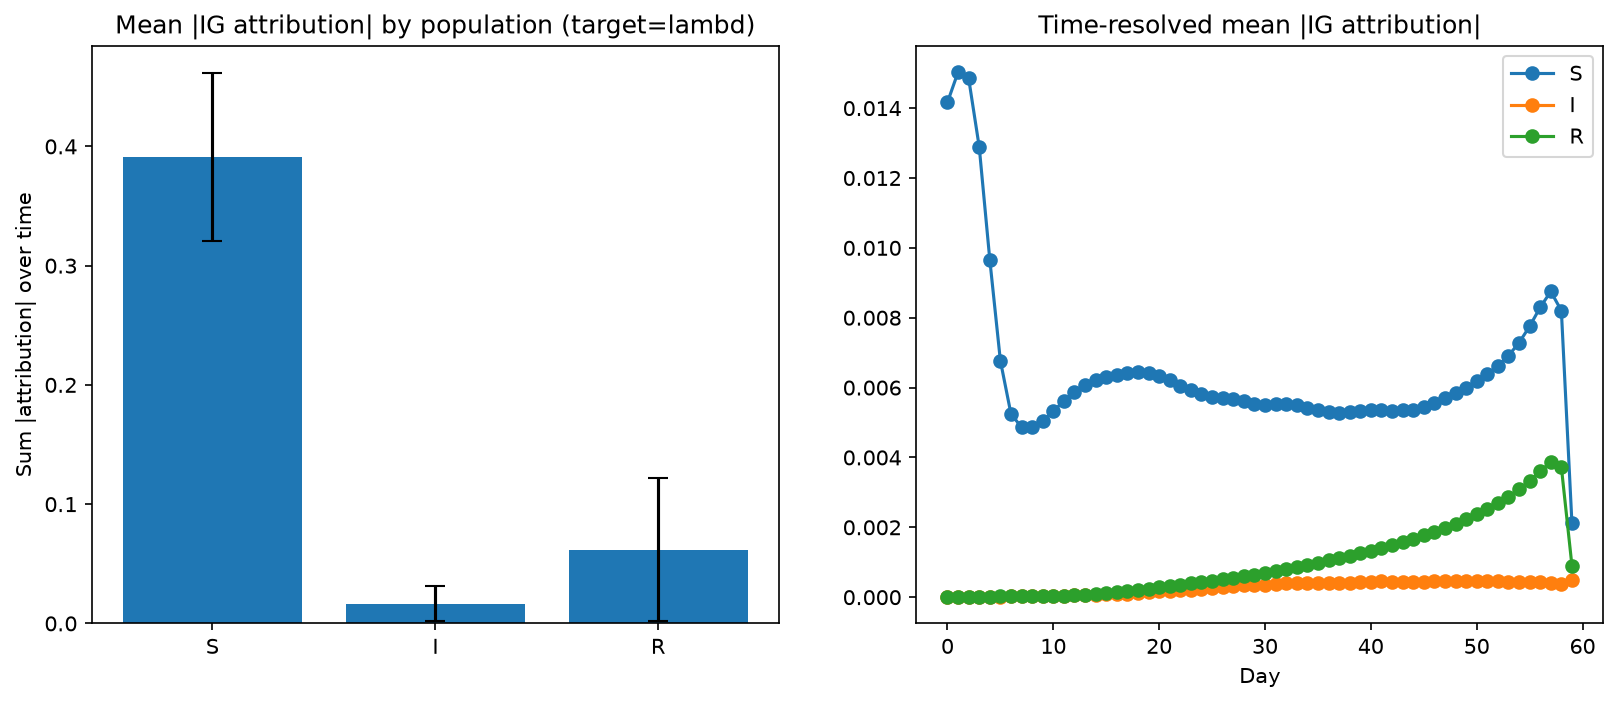
\includegraphics[width=0.9\columnwidth]{sir/xai_02_integrated_gradients.png}\\[1mm]
\begin{subfigure}{0.42\columnwidth}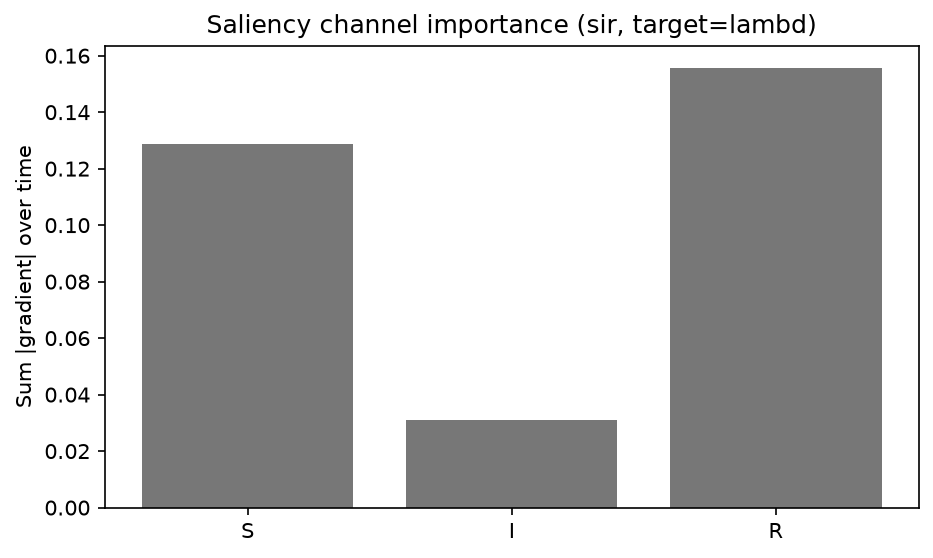
\includegraphics[width=\linewidth]{sir/workflow_sir_saliency_map_saliency_map.png}\end{subfigure}\hspace{3mm}
\begin{subfigure}{0.42\columnwidth}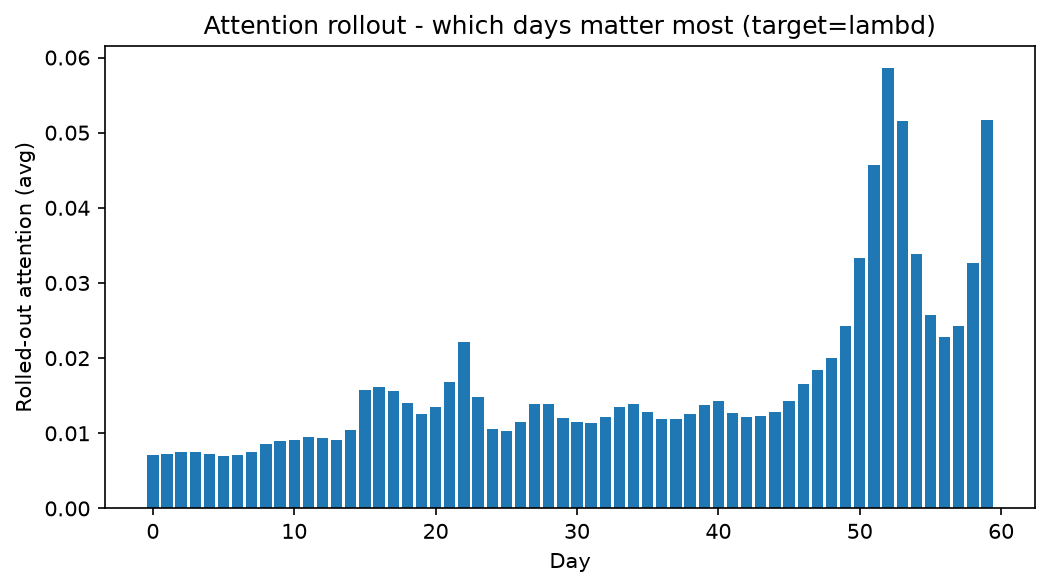
\includegraphics[width=\linewidth]{sir/xai_03a_attention_rollout_bar.png}\end{subfigure}
\caption{SIR, target $\lambda$. \textbf{Top:} IG by channel and over time. \textbf{Bottom left:} Saliency by
channel. \textbf{Bottom right:} attention rollout per day (Transformer).}
\label{fig:sir-xai}
\end{figure}

\begin{table}[t]
\centering
\caption{SIR, target $\lambda$: channel ranking and temporal focus per method.}
\label{tab:sir}
\footnotesize
\setlength{\tabcolsep}{3pt}
\begin{tabular}{@{}p{2.3cm}p{2.5cm}p{2.6cm}@{}}
\toprule
Method & Channel ranking & Temporal focus \\
\midrule
IG (200 samples) & $S\gg R>I$ \newline (0.39/0.06/0.02) & days 0--3, 50--58 \\
IG statistics (50) & $S$ dominant in 48/50 & days 1--2, 17--25, 54--59 \\
Saliency & $R>S\gg I$ \newline (0.16/0.13/0.03) & -- \\
Masking & -- & rising to last day \\
Attention rollout & -- & days 49--53, last day \\
\bottomrule
\end{tabular}
\end{table}

Table~\ref{tab:sir} and Fig.~\ref{fig:sir-xai} show that the methods disagree. Paired $t$-tests on per-sample
channel importance under IG are all significant ($p<10^{-27}$), so the dominance of $S$ is not noise. Saliency,
which lacks the factor $(x_i-x'_i)$ of Eq.~\eqref{eq:ig}, ranks $R$ first. Since $S/N\approx1$ over most of the
window while $I/N$ is a few percent, the zero baseline gives $S$ a far larger multiplier; the $S$-dominance
under IG is therefore at least partly a baseline effect~\cite{sturmfels2020baselines}. The Transformer is trained
on all five parameters jointly, so its rollout is identical for every target.

\paragraph{GRF.} Mean IG and Saliency maps for $\alpha$ are diffuse over the interior with a dark frame of a few
pixels, and $8\times8$ masking assigns the lowest importance to the outer patch columns. This matches the global
role of $\alpha$ (spatial correlation), and the dark frame is consistent with zero padding, which gives border
pixels fewer receptive fields.

\subsection{Q3: Attribution exposes a simulator artefact}

Using identical simulations (5000, data seed 0) and training, we vary only the input normalization
(Table~\ref{tab:gw-norm}, Fig.~\ref{fig:gw-norm}). With the original min-max scaling, IG concentrates in blocks
near $-0.7$, $-0.2$ and $+0.3$\,s, where the merger contributes almost nothing; no sample has its attribution peak
within $\pm50$\,ms of the merger.

\begin{table}[t]
\centering
\caption{GW, target $m_1$: effect of input normalization (64 validation samples).}
\label{tab:gw-norm}
\footnotesize
\setlength{\tabcolsep}{3pt}
\begin{tabular}{@{}lcccc@{}}
\toprule
Normalization & Val.\ MSE & IG peak & Peak $\pm$50\,ms & Last 0.2\,s \\
\midrule
min-max (orig.) & 9.27 & $-212$\,ms & \textcolor{warn}{\textbf{0\%}} & 20\% \\
z-score & \textbf{1.41} & $-4.9$\,ms & \textbf{100\%} & 40\% \\
\bottomrule
\end{tabular}
\end{table}

\begin{figure}[t]
\centering
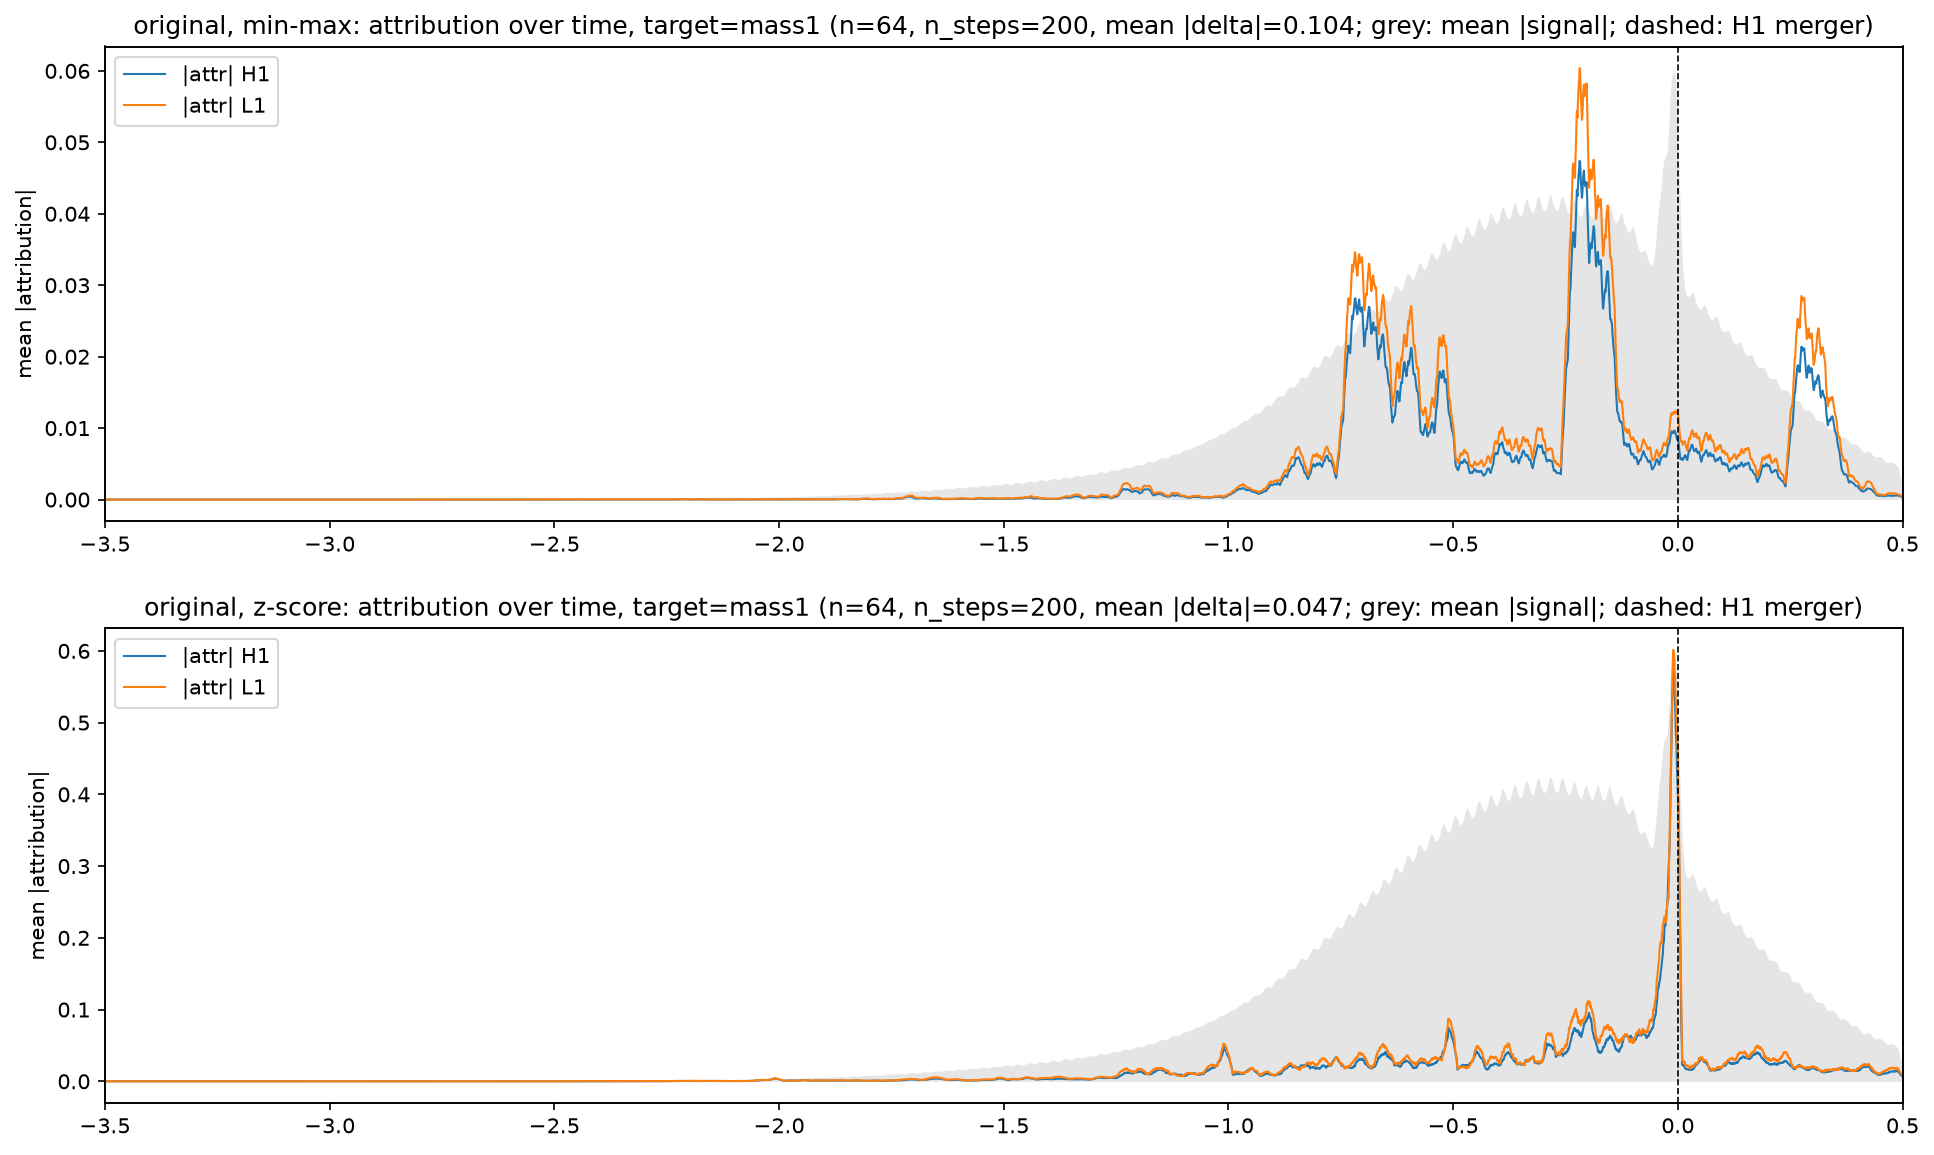
\includegraphics[width=\columnwidth]{gw_ig_time_compact.png}
\caption{GW, mean $|$IG$|$ over time (s, relative to the H1 merger) for min-max (top) and z-score inputs (bottom);
grey: mean $|$signal$|$; dashed: merger. With min-max inputs the attribution avoids the merger.}
\label{fig:gw-norm}
\end{figure}

Tracing the simulator stage by stage locates the cause. PyCBC starts the waveform below 20\,Hz, where the noise
power spectral density (PSD) is zero. Whitening estimates the PSD from the data and therefore \emph{amplifies}
the sub-20\,Hz inspiral: the standard deviation at $-1$\,s grows from 33 (whitened noise alone) to
$2.5\cdot10^5$. The 20\,Hz FIR high-pass reduces it only about sixfold. Every sample is dominated by a nearly
monochromatic ${\sim}20$\,Hz oscillation with a bell-shaped envelope from $-1.5$ to $+0.5$\,s that continues past
the merger, while the physical chirp is visible only in the last ${\sim}50$\,ms. Min-max scaling devotes almost
the full $[0,1]$ range to this artefact. The simulator was deliberately left unmodified: the artefact is a finding
of the attribution analysis, not of the loss, which trains normally.

\subsection{Comparing methods on one model}

On a z-score model (data seed 42, validation MSE 0.60), we compute IG, Saliency and Masking on the same 64
samples (Table~\ref{tab:gw-methods}). The rank correlation of the time profiles is 0.99 between IG and Masking
and 0.47 for both pairs involving Saliency. IG's mean convergence delta is 0.046, against a mean
$|f(x)-f(x')|$ of 12.3. Saliency's peaks in the signal-free window fall on a regular 0.25\,s grid
(512 samples $=2^9$, one of the embedding's dilations), suggesting an architectural origin; this is an
observation, not a tested claim.

\begin{table}[t]
\centering
\caption{GW, one z-score model: IG vs.\ Saliency vs.\ Masking. Signal energy H1/L1: 45/55.}
\label{tab:gw-methods}
\footnotesize
\setlength{\tabcolsep}{3pt}
\begin{tabular}{@{}lccc@{}}
\toprule
 & IG & Saliency & Masking \\
\midrule
Peak of mean attribution & $-5.4$\,ms & \textcolor{warn}{$-3010$\,ms} & $-10.7$\,ms \\
Peaks within $\pm$50\,ms & 97\% & \textcolor{warn}{25\%} & 100\% \\
Share in last 0.2\,s & 46\% & \textcolor{warn}{11\%} & 41\% \\
Share in $[-3.5,-1]$\,s & 7.5\% & \textcolor{warn}{58\%} & 7.8\% \\
Share after merger & 13\% & 17\% & 14\% \\
H1/L1 attribution & 57/43 & 60/40 & 59/41 \\
\bottomrule
\end{tabular}
\end{table}

%======================================================================
\section{Discussion}
%======================================================================

\paragraph{Attribution complements SBI diagnostics.} The min-max GW model trains without visible problems; only
the attribution analysis showed that it ignored the merger, and following the attribution back into the
simulator located the cause (Q3). Attribution checks \emph{what} a network learned, which recovery and
calibration on simulated data cannot.

\paragraph{Agreement is more informative than a single map.} IG and Masking agree almost perfectly on the GW
model although one integrates gradients and the other uses only forward passes. Both measure change relative to
the zero-strain baseline, so empty regions score near zero, whereas Saliency measures sensitivity, which can be
high where there is no signal---in line with known failure modes of gradient
maps~\cite{adebayo2018sanity,kindermans2019unreliability}. Where methods disagree, as on SIR (Q2), no single map
should be trusted.

\paragraph{Fingerprints of architecture and baseline.}\label{sec:fingerprints}
Several patterns stem from the model or the method rather than the data. The GRU surrogates read only the final
hidden state, so the last time step reaches the output through a single update and dominates attributions
(according to the code documentation, it is the arg-max in every sample under both a zero and a mean baseline);
endpoints are therefore excluded from the rankings. Zero baselines favour large-magnitude channels under IG;
zero padding darkens image borders; and the dilated GW embedding leaves a periodic grid in Saliency.

\paragraph{Detector preference is not robust.} The H1 preference of 57--60\% is consistent across methods for one
model, but an earlier z-score model (data seed 0) gave H1/L1 = 46/54, close to its signal energy (42/58). It is a
property of a training run, not a physical result.

%======================================================================
\section{Limitations and Future Work}
%======================================================================

\begin{itemize}
  \item \textbf{Surrogates, not posteriors.} Attributions are computed on MSE regressors, not on the BayesFlow
  summary network and flow; for SIR the surrogate also sees noise-free S/I/R instead of noisy cases.
  \item \textbf{Partial fit.} The SIR surrogate explains only $\lambda$; standardizing targets would likely help
  for $\mu$ and $D$.
  \item \textbf{Single runs.} Most results use one seed; the two z-score GW models differ by more than $2\times$
  in validation MSE.
  \item \textbf{No faithfulness metrics.} Methods are compared with each other and with known structure, not with
  deletion/insertion curves or randomization tests~\cite{adebayo2018sanity}.
  \item \textbf{Baselines.} IG used a zero baseline for SIR, the toy signal and the GRF.
\end{itemize}
Future work includes attributing through the BayesFlow summary network itself (e.g.\ to posterior moments),
multi-seed studies, quantitative faithfulness evaluation, and systematic baseline comparisons.

%======================================================================
\section{Conclusion}
%======================================================================

Attribution methods are a useful complement to standard SBI diagnostics. On a toy problem they recover the
known structure; on a realistic gravitational-wave benchmark, Integrated Gradients revealed that a network relied
on a simulator artefact rather than the physical signal, leading to a better normalization. Attributions also
depend on architecture, baseline and training run, and are best read through agreement between methods.

\paragraph{Reproducibility.} Code, configurations and figures are available at
\url{https://github.com/ferihabircan/bayesflow-xai}. During preparation of this report, a bug in the SIR
recovered-compartment update (recoveries computed from the updated rather than the previous infected count) was
fixed; it affected only the trajectories seen by the surrogates, and the SIR surrogate figures were regenerated
with unchanged qualitative results.

\small
\begin{thebibliography}{99}
\setlength{\itemsep}{1pt}
\bibitem{abnar2020quantifying} S.~Abnar and W.~Zuidema. Quantifying attention flow in transformers. In \emph{ACL}, 2020.
\bibitem{adebayo2018sanity} J.~Adebayo, J.~Gilmer, M.~Muelly, I.~Goodfellow, M.~Hardt, and B.~Kim. Sanity checks for saliency maps. In \emph{NeurIPS}, 2018.
\bibitem{ancona2018towards} M.~Ancona, E.~Ceolini, C.~\"Oztireli, and M.~Gross. Towards better understanding of gradient-based attribution methods for deep neural networks. In \emph{ICLR}, 2018.
\bibitem{cranmer2020frontier} K.~Cranmer, J.~Brehmer, and G.~Louppe. The frontier of simulation-based inference. \emph{PNAS}, 117(48), 2020.
\bibitem{dax2021realtime} M.~Dax, S.~R.~Green, J.~Gair, J.~H.~Macke, A.~Buonanno, and B.~Sch\"olkopf. Real-time gravitational wave science with neural posterior estimation. \emph{Physical Review Letters}, 127, 2021.
\bibitem{deistler2025practical} M.~Deistler et al. Simulation-based inference: A practical guide. arXiv preprint, 2025. Code: \url{https://github.com/sbi-dev/sbi-practical-guide}.
\bibitem{dinh2017realnvp} L.~Dinh, J.~Sohl-Dickstein, and S.~Bengio. Density estimation using Real NVP. In \emph{ICLR}, 2017.
\bibitem{durkan2019neural} C.~Durkan, A.~Bekasov, I.~Murray, and G.~Papamakarios. Neural spline flows. In \emph{NeurIPS}, 2019.
\bibitem{greenberg2019automatic} D.~Greenberg, M.~Nonnenmacher, and J.~Macke. Automatic posterior transformation for likelihood-free inference. In \emph{ICML}, 2019.
\bibitem{hermans2022trust} J.~Hermans, A.~Delaunoy, F.~Rozet, A.~Wehenkel, V.~Begy, and G.~Louppe. A trust crisis in simulation-based inference? Your posterior approximations can be unfaithful. \emph{TMLR}, 2022.
\bibitem{kindermans2019unreliability} P.-J.~Kindermans, S.~Hooker, J.~Adebayo, M.~Alber, K.~T.~Sch\"utt, S.~D\"ahne, D.~Erhan, and B.~Kim. The (un)reliability of saliency methods. In \emph{Explainable AI: Interpreting, Explaining and Visualizing Deep Learning}, Springer, 2019.
\bibitem{kokhlikyan2020captum} N.~Kokhlikyan et al. Captum: A unified and generic model interpretability library for PyTorch. arXiv:2009.07055, 2020.
\bibitem{lundberg2017shap} S.~M.~Lundberg and S.-I.~Lee. A unified approach to interpreting model predictions. In \emph{NeurIPS}, 2017.
\bibitem{papamakarios2016fast} G.~Papamakarios and I.~Murray. Fast $\epsilon$-free inference of simulation models with Bayesian conditional density estimation. In \emph{NeurIPS}, 2016.
\bibitem{radev2020bayesflow} S.~T.~Radev, U.~K.~Mertens, A.~Voss, L.~Ardizzone, and U.~K\"othe. BayesFlow: Learning complex stochastic models with invertible neural networks. \emph{IEEE TNNLS}, 33(4), 2022.
\bibitem{radev2021outbreakflow} S.~T.~Radev, F.~Graw, S.~Chen, N.~T.~Mutters, V.~M.~Eichel, T.~B\"arnighausen, and U.~K\"othe. OutbreakFlow: Model-based Bayesian inference of disease outbreak dynamics with invertible neural networks and its application to the COVID-19 pandemics in Germany. \emph{PLOS Computational Biology}, 17(10), 2021.
\bibitem{radev2023bayesflow} S.~T.~Radev, M.~Schmitt, L.~Schumacher, L.~Elsem\"uller, V.~Pratz, Y.~Sch\"alte, U.~K\"othe, and P.-C.~B\"urkner. BayesFlow: Amortized Bayesian workflows with neural networks. \emph{Journal of Open Source Software}, 8(89), 2023.
\bibitem{ribeiro2016lime} M.~T.~Ribeiro, S.~Singh, and C.~Guestrin. ``Why should I trust you?'' Explaining the predictions of any classifier. In \emph{KDD}, 2016.
\bibitem{simonyan2014deep} K.~Simonyan, A.~Vedaldi, and A.~Zisserman. Deep inside convolutional networks: Visualising image classification models and saliency maps. In \emph{ICLR Workshop}, 2014.
\bibitem{sturmfels2020baselines} P.~Sturmfels, S.~Lundberg, and S.-I.~Lee. Visualizing the impact of feature attribution baselines. \emph{Distill}, 2020.
\bibitem{sundararajan2017axiomatic} M.~Sundararajan, A.~Taly, and Q.~Yan. Axiomatic attribution for deep networks. In \emph{ICML}, 2017.
\bibitem{talts2018sbc} S.~Talts, M.~Betancourt, D.~Simpson, A.~Vehtari, and A.~Gelman. Validating Bayesian inference algorithms with simulation-based calibration. arXiv:1804.06788, 2018.
\bibitem{zeiler2014visualizing} M.~D.~Zeiler and R.~Fergus. Visualizing and understanding convolutional networks. In \emph{ECCV}, 2014.
\end{thebibliography}

\end{document}
